\section{Filesystems}
Filesystems are used to store data on for instance a hard drive of a computer on in the cloud. Google Drive is a filesystem that enables user to save their data online up to 15 GB for free\cite{CloudStorageWork} using their clusters of distributed storage devices, meaning that the data is saved on theirs servers which can be located wherever\cite{DistributedStorageWhat}. Paying customers can achieve higher amount of storage using the service.

A deniable filesystem is a system that does not expose files stored on this system without credentials - neither how many files are stored, their sizes, their content or even if there exists any files on the filesystem\cite{petersDEFYDeniableFile2014}. This is useful if for example one is to be exposed to an audit of their data by a totalitarian regim where they don't even want to disclose that they have data.

A unix filesystem uses a datastructure called an \textit{inode}. An inode keeps track of the metadata for the files in the filesystem, and a directory simply contains the file names, and each files/directory's inode id. Using a lookup, the system can then learn about the file - where it is located, how bit it is etc., as can be seen in Figure~\ref{fig:inode_diag} (\textbf{CITATION NEEDED}).

\begin{figure}[!ht]
	\begin{center}
	  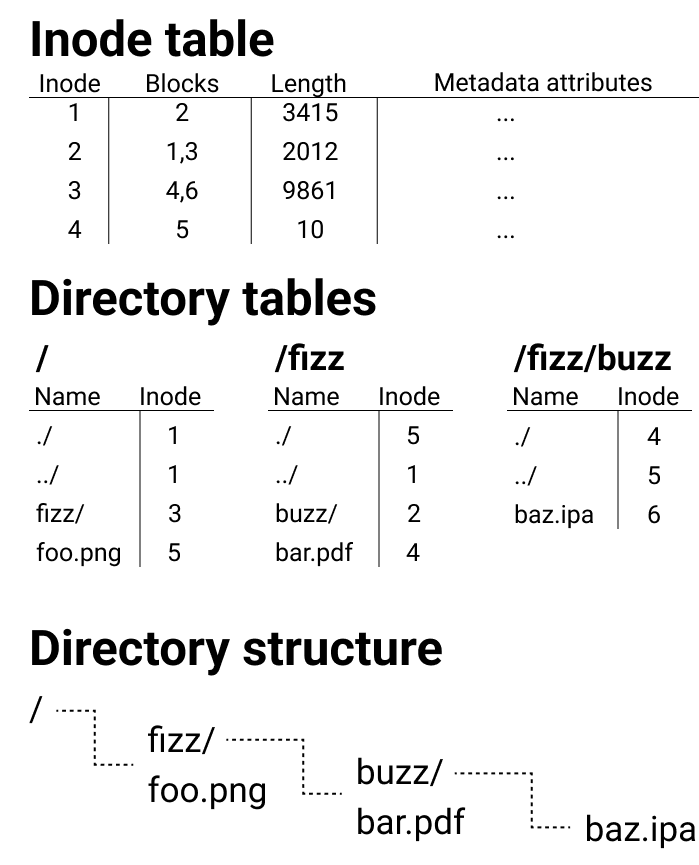
\includegraphics[width=0.8\textwidth]{figures/inode_diagram.png}
	\end{center}
	\caption{Basic structure of inode based filesystem}
	\label{fig:inode_diag}
\end{figure}
